\section{Results}
\label{sec:results}

\subsection{The home condition: 40\% symmetric noise}

\begin{table}[t]
\centering
\caption{40\% symmetric noise, all fourteen methods (5 seeds, mean $\pm$ sd). \textbf{sel}: test
accuracy at the epoch chosen on noisy held-out labels (headline). \textbf{final}: last epoch.
\textbf{best}: oracle epoch chosen on the clean test set. \textbf{mem}: corrupted probe labels
predicted as given at the last epoch. $\Delta$CE: paired sel difference to cross-entropy, with $t$.}
\label{tab:main}
\small
\renewcommand{\arraystretch}{0.95}
\begin{tabular}{llccccc}
\toprule
& method & sel & final & best (oracle) & mem & $\Delta$CE sel ($t$) \\
\midrule
\multirow{7}{*}{\rotatebox{90}{baselines}}
& CE                              & 66.97\sd{0.48} & 51.51\sd{1.22} & 67.08\sd{0.50} & 96.1 & --- \\
& GCE, $q=0.7$                    & 67.34\sd{0.78} & 65.55\sd{0.86} & 67.80\sd{0.34} & 24.3 & $+0.36$ (0.7) \\
& GCE, $q=0.4$                    & 67.20\sd{0.60} & 57.51\sd{1.41} & 67.62\sd{0.45} & 60.6 & $+0.23$ (0.6) \\
& SCE, $(0.1, 1)$                 & 66.64\sd{0.88} & 63.07\sd{0.75} & 67.69\sd{0.28} & 29.1 & $-0.33$ ($-0.7$) \\
& SCE, $(1, 1)$                   & 66.73\sd{0.69} & 54.62\sd{1.16} & 67.50\sd{0.56} & 75.6 & $-0.24$ ($-0.6$) \\
& small-loss, $r = \eta$ (oracle) & 65.61\sd{1.19} & 64.38\sd{0.94} & 67.10\sd{0.33} & 25.9 & $-1.37$ ($-2.3$) \\
& small-loss, $r = \eta/2$        & 66.75\sd{1.13} & 58.70\sd{0.63} & 67.11\sd{0.57} & 58.2 & $-0.22$ ($-0.5$) \\
\midrule
\multirow{4}{*}{\rotatebox{90}{\scriptsize batch-rel.}}
& AS-Softmax ($\beta = 0$)        & 66.71\sd{0.91} & 53.42\sd{0.64} & 67.40\sd{0.47} & 96.4 & $-0.26$ ($-0.7$) \\
& M4, $\beta = 0.25$              & 66.74\sd{0.99} & 53.04\sd{2.74} & 67.43\sd{0.54} & 96.0 & $-0.24$ ($-0.4$) \\
& M4, $\beta = 0.5$               & 66.84\sd{0.63} & 58.49\sd{1.47} & 67.19\sd{0.54} & 53.8 & $-0.14$ ($-0.5$) \\
& M4, $\beta = 1$                 & \textbf{67.44}\sd{0.55} & \textbf{66.72}\sd{0.80} & 67.64\sd{0.28} & 16.1 & $+0.47$ (1.4) \\
\midrule
\multirow{3}{*}{\rotatebox{90}{\scriptsize self-calib.}}
& absolute gap, $\tau = 0.1$      & 66.39\sd{0.65} & 65.93\sd{1.01} & 67.01\sd{0.44} & \textbf{9.5} & $-0.59$ ($-1.8$) \\
& absolute gap, $\tau = 0.3$      & 66.56\sd{1.15} & 52.58\sd{1.57} & 67.23\sd{0.49} & 95.6 & $-0.41$ ($-0.8$) \\
& loss mixture                    & 65.33\sd{0.90} & 64.55\sd{0.34} & 66.26\sd{0.53} & 23.1 & $-1.64$ ($-3.0$) \\
\bottomrule
\end{tabular}
\end{table}

\Cref{tab:main} gives the condition the batch-relative margin was designed around. Four
observations stand out.

\emph{Model selection on noisy labels compresses everything.} Under sel, twelve of the fourteen
methods fall within 0.8 points of CE, and none is established as better than CE. Early stopping on
noisy held-out labels already captures most of what robust training buys at this noise rate. The
differences reappear without selection: at the last epoch CE has dropped to 51.5\%, and the two
rejection margins hold 66.7\% (batch-relative) and 65.9\% (absolute), above GCE (65.6) and
small-loss (64.4).

\emph{The absolute margin memorizes least.} It ends training having fitted 9.5\% of the
corrupted probe labels. That is the lowest of all fourteen methods, against 24--26\% for GCE and
oracle small-loss and 96\% for CE. It does so without being told the noise rate.

\emph{The strength sweep is a threshold, as \cref{prop:reject} predicts.} Memorization goes
96 / 96 / 54 / 16\% for $\beta = 0 / 0.25 / 0.5 / 1$. The cap $\beta - \dbase$ explains the shape.
At $\beta = 0.25$ only gaps below 0.10 are rejectable, while the mislabeled samples' gaps are
large once early learning has happened. The same geometry predicts the failure of the
absolute gap at $\tau = 0.3$. Its band $[0.26, 0.64]$ lets the most contradicted labels escape,
and it memorizes like AS-Softmax (95.6\%).

\emph{Estimating the rate is not enough.} The loss-mixture statistic estimates the noise rate well
(0.35 $\pm$ 0.01 against a true 0.40) but is the least accurate margin, 1.64 points below CE
($t = -3.0$). It also memorizes more than the absolute rule (23\% vs.\ 9.5\%). Knowing \emph{how
many} labels are wrong did not tell it \emph{which}.

\subsection{Across noise conditions}

\begin{table}[t]
\centering
\caption{All six conditions for the five main methods (5 seeds, mean $\pm$ sd). Top: test accuracy
with noisy-held-out selection. Middle: last epoch. Bottom: memorization of corrupted labels at the
last epoch (\%). Small-loss equals CE at $\eta = 0$ ($r = 0$). Small-loss is given the true rate.}
\label{tab:conditions}
\small
\setlength{\tabcolsep}{4.5pt}
\begin{tabular}{lcccccc}
\toprule
& \multicolumn{4}{c}{symmetric} & \multicolumn{2}{c}{pair-flip} \\
\cmidrule(lr){2-5}\cmidrule(lr){6-7}
method & 0\% & 20\% & 40\% & 60\% & 20\% & 40\% \\
\midrule
\multicolumn{7}{l}{\emph{sel (noisy held-out selection)}} \\
CE              & \textbf{71.38}\sd{0.61} & 68.34\sd{0.80} & 66.97\sd{0.48} & 63.65\sd{0.99} & 67.39\sd{1.48} & 57.31\sd{4.79} \\
small-loss      & \textbf{71.38}\sd{0.61} & 68.72\sd{0.83} & 65.61\sd{1.19} & 63.41\sd{1.24} & 67.62\sd{0.64} & 59.42\sd{2.35} \\
GCE             & 71.15\sd{0.39} & \textbf{68.86}\sd{0.27} & 67.34\sd{0.78} & \textbf{64.55}\sd{0.51} & \textbf{68.16}\sd{0.52} & 57.76\sd{6.15} \\
M4 (batch-rel.) & 67.55\sd{1.27} & 68.49\sd{0.51} & \textbf{67.44}\sd{0.55} & 62.52\sd{1.37} & 66.93\sd{0.66} & 52.71\sd{3.65} \\
absolute gap    & 69.88\sd{0.37} & 67.83\sd{0.66} & 66.39\sd{0.65} & 63.27\sd{1.03} & 68.04\sd{0.52} & \textbf{62.69}\sd{1.55} \\
\midrule
\multicolumn{7}{l}{\emph{final (last epoch)}} \\
CE              & \textbf{71.25}\sd{0.14} & 62.94\sd{0.68} & 51.51\sd{1.22} & 36.89\sd{1.57} & 61.96\sd{1.37} & 48.95\sd{1.39} \\
small-loss      & \textbf{71.25}\sd{0.14} & 67.39\sd{0.91} & 64.38\sd{0.94} & 61.99\sd{0.39} & 65.33\sd{0.87} & 53.63\sd{2.61} \\
GCE             & 70.85\sd{0.52} & \textbf{68.91}\sd{0.33} & 65.55\sd{0.86} & 57.24\sd{0.60} & \textbf{67.35}\sd{0.78} & 49.32\sd{0.71} \\
M4 (batch-rel.) & 64.43\sd{2.25} & 68.51\sd{0.55} & \textbf{66.72}\sd{0.80} & 54.92\sd{2.07} & 64.98\sd{0.70} & 47.19\sd{1.85} \\
absolute gap    & 68.75\sd{0.89} & 67.60\sd{0.90} & 65.93\sd{1.01} & \textbf{62.38}\sd{1.55} & 66.43\sd{1.18} & \textbf{56.44}\sd{5.13} \\
\midrule
\multicolumn{7}{l}{\emph{memorization at the last epoch (\%)}} \\
CE              & --- & 93.5 & 96.1 & 97.4 & 96.6 & 97.1 \\
small-loss      & --- & 29.4 & 25.9 & 13.4 & 50.9 & 48.5 \\
GCE             & --- & 16.1 & 24.3 & 31.4 & 39.3 & 80.4 \\
M4 (batch-rel.) & --- & \textbf{7.0} & 16.1 & 32.6 & 34.3 & 66.5 \\
absolute gap    & --- & 9.3 & \textbf{9.5} & \textbf{8.0} & \textbf{17.5} & \textbf{26.3} \\
\bottomrule
\end{tabular}
\end{table}

\begin{figure}[t]
  \centering
  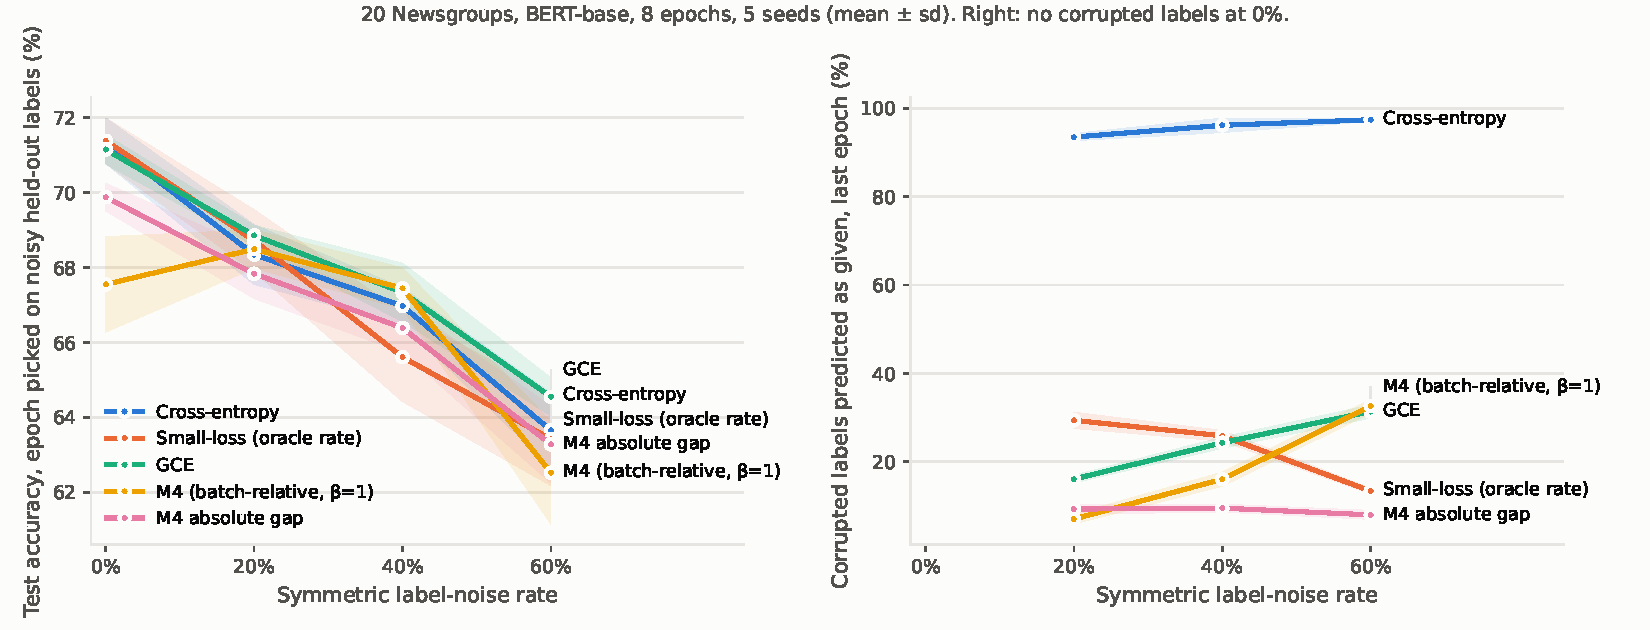
\includegraphics[width=\linewidth]{figures/figC1_noise_curves.pdf}
  \caption{Symmetric noise. Left: test accuracy with noisy-held-out selection. Right: memorization
  of corrupted labels at the last epoch. Mean $\pm$ sd over 5 seeds. The batch-relative margin
  (yellow) is competitive only near 40\%, the rate its fixed strength suits. The absolute margin
  (pink) keeps memorization at 8--10\% at every rate.}
  \label{fig:noise}
\end{figure}

\begin{figure}[t]
  \centering
  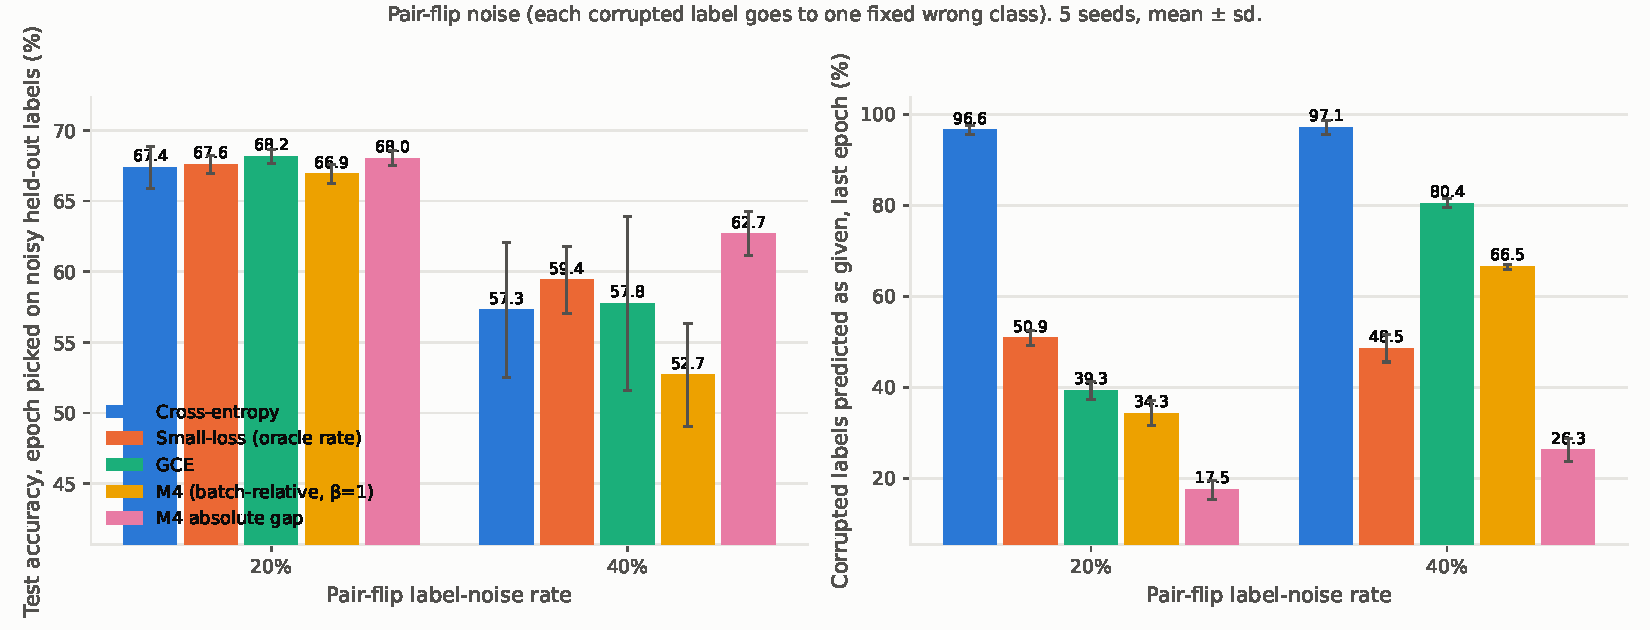
\includegraphics[width=\linewidth]{figures/figC2_pair_noise.pdf}
  \caption{Pair-flip noise, where each corrupted label goes to one fixed wrong class. The absolute
  margin is the only method whose accuracy holds at 40\% and the only one that keeps memorization
  well below half.}
  \label{fig:pair}
\end{figure}

\Cref{tab:conditions} and \cref{fig:noise,fig:pair} test the two statistics' predictions away
from the home condition.

\emph{The batch-relative margin is noise-blind, as \cref{prop:blind} predicts.} On clean data it
loses 3.83 points to CE (5/5 seeds, $t = -5.2$), and 6.8 at the last epoch: it keeps discarding
correctly labeled samples that are merely below their batch's average. At 60\% symmetric noise it
under-rejects (memorization 33\%, twice its 40\% level) and trails GCE by 2.0 points ($t = -3.4$).
Under 40\% pair-flip noise it is the worst method, 4.6 points below CE ($t = -2.0$) and 6.7 below
small-loss ($t = -3.6$). The strength that suits 40\% symmetric noise is a hidden rejection rate
that suits nothing else.

\emph{The absolute margin follows the data, but pays on easy regimes.} Its clean-data cost falls
from 3.83 to 1.51 points; that is still established ($t = -5.1$), so P1 fails. Under structured
noise it is the best method: at 40\% pair-flip it reaches 62.69, $+5.38$ over CE ($t = 3.4$, 5/5
seeds) and $+3.27$ over small-loss given the true rate ($t = 3.3$). It is $+4.93$ over GCE, though
GCE's variance across seeds is too large to establish that ($t = 1.7$). Its memorization there
(26\%) is half of small-loss's and a third of GCE's. On symmetric noise it trails GCE by 1.0
($\eta = 0.2$, $t = -3.4$), 0.95 ($\eta = 0.4$, $t = -1.9$) and 1.3 points ($\eta = 0.6$,
$t = -2.1$). The rule rejects every sample the model currently disagrees with. That includes hard
but correctly labeled samples, and on easy regimes GCE's soft down-weighting is the better trade.

\emph{Without a validation set, the absolute margin's advantage grows with the noise.} At the last
epoch its difference to GCE goes from $-2.1$ (clean) and $-1.3$ (20\%) to $+0.4$ (40\%),
$+5.1$ (60\%, $t = 9.7$, 5/5 seeds) and $+7.1$ (pair 40\%, $t = 3.1$). Under symmetric noise the
absolute margin loses at most 0.9 points between the selected and the last epoch (GCE: up to 7.3),
because it keeps refusing to fit what it disagrees with. Under pair-flip noise both decay more
(absolute gap 6.3, GCE 8.4 points at 40\%).

\subsection{Pre-registered verdicts}

\begin{table}[t]
\centering
\caption{Pre-registered criteria (fixed before the corresponding runs) and outcomes. Accuracies
use sel unless noted. N1--N4 were defined for the batch-relative M4 (Phases A--C), P1--P4 for the
self-calibrating statistics (Phase C$'$). The loss mixture was eliminated at P3 and, by the
pre-registered rule, not run elsewhere.}
\label{tab:verdicts}
\small
\begin{tabular}{p{0.24\linewidth}p{0.42\linewidth}p{0.24\linewidth}}
\toprule
criterion & outcome & verdict \\
\midrule
N1 replicate (4 ep., final) & M4 $-$ CE $= +1.81$, $t = 4.4$, 5/5 seeds; memorization 17\% vs.\ 35\% & pass \\
N2 $\ge$ small-loss $-$ 0.5 & 4 ep.\ final: $-0.39$ after removing the timing confound (B$'$); 8 ep.\ sel: $+1.84$ & pass \\
N3 $\ge \max$(GCE, SCE) & 4 ep.\ final: $-0.49$ vs.\ GCE; 8 ep.\ sel: $+0.11$ & fail at 4 ep., tie at 8 \\
N4 memorization falls steadily in $\beta$ & 96 / 96 / 54 / 16\%: monotone, threshold-shaped (\cref{prop:reject}) & partial \\
\midrule
P1 clean cost $\ge$ CE $-$ 0.5 & absolute gap $-1.51$ ($t = -5.1$) & fail \\
P2 adaptivity & masked-slot ratio flat (0.996) at every rate; mixture estimate 0.35 at $\eta = 0.4$ & fail as worded \\
P3 home $\ge$ best baseline $-$ 0.5 $= 66.84$ & absolute gap 66.39; mixture 65.33 & fail (both) \\
P4 pair 40\%: $\ge$ CE, within 2 of small-loss & absolute gap 62.69 vs.\ 57.31 / 59.42 & pass \\
\bottomrule
\end{tabular}
\end{table}

\Cref{tab:verdicts} collects the pre-registered tests. The decisive one is P3. The bar was the best
tuned baseline at the home condition minus half a point, $67.34 - 0.5 = 66.84$, and neither
self-calibrating statistic reached it. By the rule we fixed in advance, the absolute-gap margin is
therefore not presented as a new method, and the real-noise benchmark (CIFAR-10N/100N,
\citealp{wei2022cifarn}) was not run. P2 failed for a reason we only understood afterwards. Its
measure, the fraction of masked non-target slots, is dominated by AS-Softmax's masking of fitted
samples (0.996 for every method in the family at every noise rate), so it cannot register sample-level
adaptivity. The sample-level evidence is the flat 8--10\% memorization across symmetric noise rates
in \cref{tab:conditions}, against small-loss's 29\% $\to$ 13\%. We report P2 as failed, as worded.

\subsection{Mechanism}
\label{sec:mechanism}

\begin{figure}[t]
  \centering
  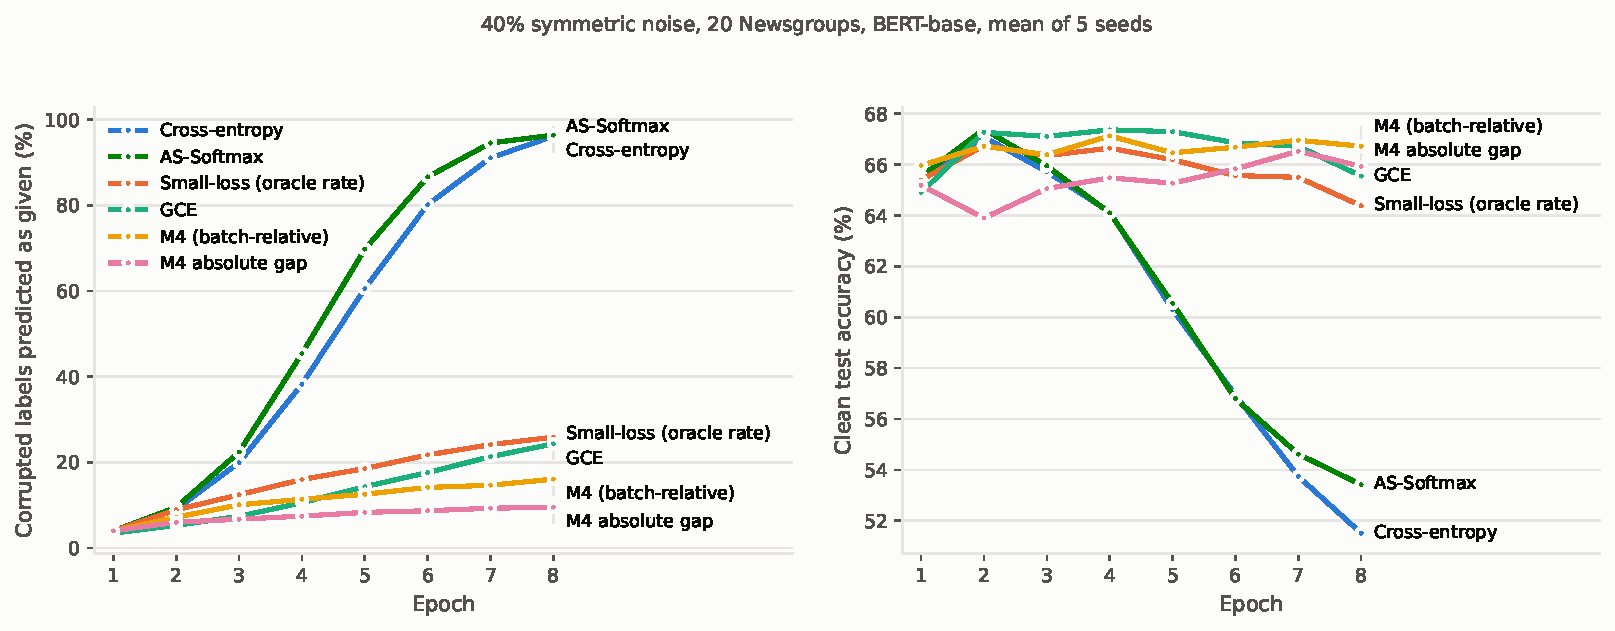
\includegraphics[width=\linewidth]{figures/fig4_dynamics.pdf}
  \caption{40\% symmetric noise, per epoch, mean of 5 seeds. Left: memorization of corrupted labels.
  AS-Softmax (green) memorizes faster than cross-entropy at epochs 3--7, on every seed. Right: clean
  test accuracy, the degradation that noisy-held-out selection has to catch.}
  \label{fig:dynamics}
\end{figure}

\paragraph{AS-Softmax memorizes faster than cross-entropy.}
\Cref{obs:as} predicts that zeroing the gradient of fitted samples shifts each update toward the
unfitted, mostly mislabeled ones. \Cref{fig:dynamics} confirms the prediction. AS-Softmax's
memorization exceeds CE's at epochs 3 through 7 on all five seeds: by 2.5 points at epoch 3
($t = 3.5$), 7.2 at epoch 4 ($t = 5.5$), 9.2 at epoch 5 ($t = 13.0$), 6.5 at epoch 6 and 3.5 at
epoch 7. Both saturate at 96\% by epoch 8. The same holds in the earlier 4-epoch runs (39.4\% vs.\
34.7\% at the last epoch). On its own, the base loss of the margin family is \emph{less}
noise-robust than cross-entropy. As a base for rejection it is nonetheless the better choice. In a
Phase~B$'$ control with identical rejection decisions, training the kept samples with CE instead of
AS-Softmax cost 4.1 points (63.3 vs.\ 67.4, 4 epochs, \cref{app:prereg}). We have not isolated why.

\paragraph{Where the gradient goes.}
\TODO{Fill from \texttt{runs/mechanism/summary.md} once the 42 instrumented runs finish (3 seeds;
the instrumentation reproduces Phase~C's accuracies exactly). Report, at the last epoch of 40\%
symmetric noise: the share of gradient carried by mislabeled probe samples for CE / AS / M4 /
absolute gap / small-loss / GCE; the fraction of mislabeled samples rejected (zero gradient with
$g > 0$); the fraction of clean samples with zero gradient at 0\% noise for M4 vs.\ absolute gap
(the clean-cost mechanism of \cref{prop:blind}); and the share of the mislabeled samples' gradient
in the escape region $g \ge 0.8$ (\cref{prop:reject}). Insert \texttt{fig5\_mechanism.pdf}.}
